\documentclass[titlepage = firstcover]{scrartcl}
\usepackage[aux]{rerunfilecheck}
\usepackage{fontspec}
\usepackage[main=ngerman, english, french]{babel}

% mehr Pakete hier
\usepackage{expl3}
\usepackage{xparse}

%Mathematik------------------------------------------------------
\usepackage{amsmath}   % unverzichtbare Mathe-Befehle
\usepackage{amssymb}   % viele Mathe-Symbole
\usepackage{mathtools} % Erweiterungen für amsmath
\usepackage[
  math-style=ISO,    % \
  bold-style=ISO,    % |
  sans-style=italic, % | ISO-Standard folgen
  nabla=upright,     % |
  partial=upright,   % /
]{unicode-math}% "Does exactly what it says on the tin."
\usepackage[section, below]{placeins}

% Laden von OTF-Mathefonts
% Ermöglich Unicode Eingabe von Zeichen: α statt \alpha

\setmathfont{Latin Modern Math}
%\setmathfont{Tex Gyre Pagella Math} % alternativ zu Latin Modern Math
\setmathfont{XITS Math}[range={scr, bfscr}]
\setmathfont{XITS Math}[range={cal, bfcal}, StylisticSet=1]

\AtBeginDocument{ % wird bei \begin{document}
  % werden sonst wieder von unicode-math überschrieben
  \RenewDocumentCommand \Re {} {\operatorname{Re}}
  \RenewDocumentCommand \Im {} {\operatorname{Im}}
}
\usepackage{mleftright}
\setlength{\delimitershortfall}{-1sp}

%Sprache----------------------------------------------------------
\usepackage{microtype}
\usepackage{xfrac}
\usepackage[autostyle]{csquotes}    % babel
\usepackage[unicode, pdfusetitle]{hyperref}
\usepackage{bookmark}
\usepackage[shortcuts]{extdash}
%Einstellungen hier, z.B. Fonts
\usepackage{booktabs} % Tabellen


\title{Der Compton-Effekt}
\author{
  Lasse Sternemann\\
  \href{mailto:lasse.sternemann@udo.edu}{lasse.sternemann@udo.edu}
}
\date{Bearbeitet am 01.05.2020}

\begin{document}
    \maketitle
    \newpage
    \tableofcontents
    \newpage
     
    \section{Zielsetzung}
    Im Experiment zum Compton-Effekt soll die Compton-Wellenlänge über die Differenz von ungestreuten Photonen und um 90° gestreuten Compton-Photonen
    bestimmt werden. 


    \section{Theoretische Grundlagen}
        \subsection{Compton-Effekt}
        Wenn ein Photon auf ein freies Elektron trifft, findet ein quasi elastischer Stoß statt. Dabei wird ein Teil des Impulses sowei ein Teil der 
        Energie des Photons an das Elektron übertragen. Aufgrund des Energieverlustes des Photons vergrößert sich dessen Wellenlänge. Dies ist in 
        Gleichung \ref{eqn:EPhoton} zu sehen.

        \begin{equation}
            E_{\text{Photon}} = \frac{hc}{\lambda}
            \label{eqn:EPhoton}
        \end{equation}
        \noindent

        Die Differenz der Wellenlängen des Photons vor $\lambda _1$ und nach dem Stoß $\lambda _2$ lässt sich über die beim elastischen Stoß geltenden
        Impuls- und Energierhaltung nach Gleichung \ref{eqn:ComptonWellenlänge} berechnen.

        \begin{equation}
            \Delta \lambda = \lambda_1 - \lambda_2 = \frac{h}{c \cdot m_e} \cdot \left(1-cos(\theta)\right) = \lambda_{\text{C}} \cdot \left(1-cos(\theta)\right)
            \label{eqn:ComptonWellenlänge}
        \end{equation}
        \noindent

        Dabei bezeichnet $\lambda_{\text{C}}$ die Compton Wellenlänge, die eine konstante ist. Aus der Gleichung lässt sich erkennen, dass die 
        Wellenlängendifferenz und somit die vom Photon abgegebene Energie vom Streuwinkel $\theta$ \ref{fig:SkizzeCompton} abhängt. Die Wellenlängendifferenz 
        wird für einen Streuwinkel von $\pi$, was einer Reflexion entspricht, maximal. Für einen gegen Null laufenden Streuwinkel geht auch die 
        Wellenlängendifferenz gegen Null und die Compton-Streuung tritt quasi nicht mehr auf.
        \begin{align}
            \Delta \lambda_{\text{max}} = 2 \cdot \lambda_{\text{C}} \qquad \text{bei} \theta = \pi \\
            \Delta \lambda_{\text{min}} \longrightarrow 0 \qquad \text{für} \theta \longrightarrow 0
        \end{align}
        \noindent

        \FloatBarrier
        \begin{figure}[h]
            \centering
            \caption{In der Abbildung ist der Compton Effekt skizziert. Der eingezeichnete Winkel $\theta$ ist der Streuwinkel des Photons.}
            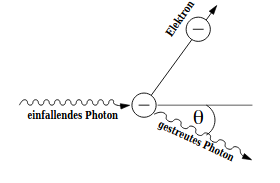
\includegraphics{SkizzeCompton.png}
            \label{fig:SkizzeCompton}
        \end{figure}
        \FloatBarrier
        \noindent

        Dieser Effekt kann für Photonen aller Energien beobachtet werden. Für hochenergetische Photonen, wie zum Beispiel Röntgen- oder $\gamma$ -Strahlung,
        ist die Wahrscheinlichkeit den Effekt zu beobachten jedoch höher.  

        \subsection{Röntgenstrahlung}
        Die für den Versuch verwendete Röntgenstrahlung wird in einer Röntgenröhre erzeugt. Dazu werden zunächst Elktronen über eine Heizspannung aus einem
        Glühdraht hinausgelöst und dann durch eine Spannung beschleunigt. Die so beschleunigten Elektronen treffen auf eine Anode und es wird Röntgenstrahlung
        ausgesendet. Das ausgesendete Spektrum setzt sich aus charakteristischen Peaks und einem kontinuierlichen Bremsspektrum zusammen. 
        
            \subsubsection*{Bremsspektrum}
                Das kontinuierliche Bremsspektrum entsteht, wenn die Elktronen sich dem Kern eines Kathodenatoms nähern und dabei durch dessen elktrisches 
                Feld abgebremst werden. Da den Elektronen hierbei eine Beschleunigung widerfährt, verlieren sie ihre kinetische Energie und senden diese als 
                Röntgenphoton aus. Die kleinste Wellenlänge entspricht dabei der Bremsstrahlung der schnellsten Elektronen und hängt von der 
                Beschleunigungsspannung ab.
                
            \subsubsection*{Charakteristische Strahlung}
                Zu der Bremsstrahlung kommen noch Peaks, die vom Anodenmaterial abhängen. Sie entstehen, wenn ein Elektron des Atoms des Kathodenmaterials 
                auf ein höheres Energieniveau angeregt wird und dann wieder auf eine niedrigeres Energieniveau zurückspringt. Dabei wird exakt die 
                Energiedifferenz zwischen den beiden Energieniveaus als Röntgenquant abggestrahlt und es entsteht ein Peak im Spektrum.
                
        \subsection{Bragg-Reflexion}
        Um im Experiment die Wellenlänge der Röntgenstrahlung zu bestimmen wird von der Bragg-Reflexion Gebrauch gemacht. Bei dieser fällt Röntgenstrahlung
        auf ein Material mit Gitterstruktur und wird dabei an den einzelnen Atomen gebeugt. Die Röntgenstrahlung interferiert nun mit sich selbst innerhalb 
        des Gitters. Die zugehörige konstruktive Interfenrenz findet sich beim Bragg-Winkel $\alpha $ \ref{fig:SkizzeBragg}, der über Formel \ref{eqn:Bragg} 
        mit der Wellenlänge der einfallenden Röntgenstrahlung verknüpft ist. Die notwendige Gitterstruktur ist zum Beispiel in Kristallen gegeben.

        \begin{equation}
            2 \cdot d \cdot sin(\alpha) = n \cdot \lambda = n \cdot \frac{hc}{E}
            \label{eqn:Bragg}
        \end{equation}

        \noindent
        Der Abstand zwischen den Atomen im Gitter fließt über die Gitterkonstante d \ref{fig:SkizzeBragg} in die Formel ein.
        
        \FloatBarrier
        \begin{figure}[h]
            \centering
            \caption{In der Abbildung ist die Bragg-Reflexion skizziert. Der Winkel $\alpha$ ist der Bragg-Winkel und d die Gitterkonstante.}
            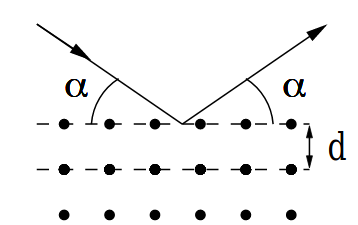
\includegraphics{Bragg.png}
            \label{fig:SkizzeBragg}
        \end{figure}
        \FloatBarrier

        \subsection{Geiger-Müller-Zählrohr}
        Zur Messung der Impulsrate wird ein Geiger-Müller-Zählrohr genutzt. Dieses besteht aus einem mit gefülltem Zylinder, dessen Wand eine große
        Kathode ist. Im Zentrum des Zylinders befindet sich eine Stabanode. Wenn nun ionisierende Strahlung in den Zylinder strahlt, treffen die Photonen
        auf Gasatome und ionisieren diese. Die dabei frei werdenden Elektronen treffen auf den Anodenmantel und werden als einzelner Impuls regestriert. Jedes
        ionisierte Gasatom wandert zur Stabanode, um neutral geladen zu werden und so wieder ionisierbar zu sein. Daraus folgt das Problem der Totzeit. Es 
        tritt auf, wenn die Intensität der Strahöung so hoch ist, dass alle Atome ionisiert sind und so nicht die gesamte Intensität gemessen wird. So würde die
        gemessene Intensität trotz kontinuierlich steigender Strahlungsintensität gegen einen Grenzwert laufen. Dieser Effekt wird über die Totzeitkorrektur 
        \ref{eqn:Totzeitkorrektur} behoben. Dabei beschreibt N die Impulsrate und $\tau$ die Totzeit.
        
        \begin{equation}
            I = \frac{N}{1-\tau \cdot N}
            \label{eqn:Totzeitkorrektur}
        \end{equation}
        

    \section{Durchführung}
        \subsection{Aufnahme des Röntgenspektrums}
        Um die für den Compton-Effekt notwendige Röntgenstrahlung zu erzeugen, wird eine Röntgenröhre benutzt, die wie bereits beschrieben ein ganzes 
        Spektrum an Röntgenstrahlung aussendet. In diesem Fall verwendet die Röntgenröhre eine Kupferanode zur Röntgenerzeugung. Um das Spektrum der 
        erzeugten Röntgenstrahlung darzustellen, wird ein Lithiumfluoridkristall in einem Winkel in den Röntgenstrahl gestellt. Das Geiger-Müller-Zählrohr
        wird im doppelten Winkel des Kristalls zu diesem ausgerichtet. So wird die Bragg-Reflexion ausgenutzt und das Geiger-Müller-Zählrohr misst nur die
        Impulsrate eines speziellen Braggwinkels, dem über Formel \ref{eqn:Bragg} eine Wellenlänge des Röntgenspektrums zugeordnet werden kann. Die Messreihe
        wird in 0,1° Schritten von 8° bis 25° aufgenommen und soll so das gesamte Bremsspektrum, sowie die charakteristischen Peaks aufnehmen.
        
        \subsection{Bestimmung der Wellenlängenabhängigkeit der Transmission}
        Für die spätere Bestimmung der Compton-Wellenlänge muss zunächst die Abhängigkeit der Transmission von der Wellenlänge bestimmt werden. Dazu wird dem
        Aufbau zur Aufnahme des Röntgenspektrums ein Aluminium-Absorber hinzugefügt, der zunächst vor der Blende der Röntgenröhre platziert wird. Dann wird 
        wieder der Anstellwinkel des Kristalls zum Röntgenstrahl von 7° bis 10° in 0,1° Schritten variiert und dabei die Intensität der Bragg reflektierten
        Strahlung gemessen. Dieselbe Messung wird ohne eingesetzten Aluminium-Absorber wiederholt, um in der Auswertung die Transmission des Aluminium-
        Absorbers zu bestimmen.

        \subsection{Bestimmung der Compton-Wellenlänge}
        Bei der Messung der Intensität der compton-gestreuten Photonen werden nur die um 90° gestreuten Photonen gemessen, indem das Geiger-Müller-Zählrohr
        in eben jenen 90° Grad zum Röntgenstrahl platziert wird \ref{fig:SkizzeAbsorber}. 
        Zunächts muss die Grundintensität $I_0$ der compton gestreuten Photonen aus der Röntgenröhre gemessen werden. Dazu wird ohne Einsatz eines Absorbers
        die an einem Plexiglas gestreute Röntgenstrahlung gemessen. Der Plexiglas-Streuer wird dazu in einem 45° Winkel in dem Röntgenstrahl platziert und es 
        wird eine Intensität aufgenommen. Daraufhin wird der Aluminium-Absorber vor die Blende gesetzt \ref{fig:SkizzeAbsorber} und bei restlich gleich bleibendem Aufbau wieder
        eine Intensität $I_1$ gemessen. Zuletzt wird der Aluminium-Absorber zwischen das Geiger-Müller-Zählrohr und den Plexiglas-Streuer gesetzt  
        \ref{fig:SkizzeCompton} und wieder bei restlich gleich bleibendem eine Intensität $I_2$ gemessen.

        \FloatBarrier
        \begin{figure}[h]
            \centering
            \caption{In der Abbildung ist der Aufbau zur Messung der Intensitäten der gestreuten Strahlung zu sehen. Während in Teil a) der Aufbau zur Messung von $I_1$ und in Teil b) der zu $I_2$ dargestellt ist, entspricht der Aufbau zur Messung $I_0$ beiden gezeigten bei Entfernung des Aluminium-Absorbers.}
            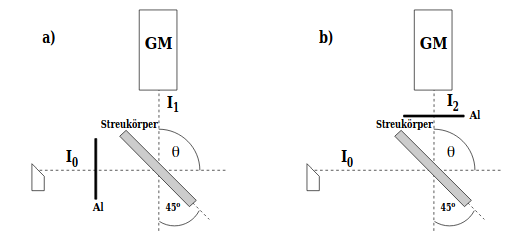
\includegraphics[width = 0.8\linewidth]{absorber.png}
            \label{fig:SkizzeAbsorber}
        \end{figure} 
        \FloatBarrier
        \newpage


    \newpage
    \section{Auswertung}
        \subsection{Röntgenspektrum}
        Zunächst werden die zur $K_{\alpha}$ und zur $K_{\beta}$ gehörigen Wellenlängen über die literarischen Werte der zugehörigen Energien (ref) 
        berechnet, indem Formel \ref{eqn:EPhoton} nach der Wellenlänge umgestellt wird.

        \begin{align}
            \lambda &= \frac{hc}{E_{K_{\alpha}}} \approx 1,6 \cdot 10^{\left(-10\right)}\,m \qquad \text{mit} \, E_{K_{\alpha}}=8038 \, \text{eV} \\
            \lambda &= \frac{hc}{E_{K_{\beta}}} \approx 1,4 \cdot 10^{\left(-10\right)}\,m \qquad \text{mit} \, E_{K_{\beta}}=8905 \, \text{eV}
        \end{align}

        \noindent
        Zudem werden die Bragg-Winkel ausgerechnet, bei denen die zu der $K_{\alpha}$ und zur $K_{\beta}$ gehörigen Wellenlängen bragg refklektiert werden, 
        sodass die Linien später einfacher im Diagramm identifiziert und verglichen werden können. Dazu wird die Bragg-Bedingung \ref{eqn:Bragg} bei n=1 
        nach $\alpha$ umgestellt. Bei Verwendung eines Lithiumfluoridkristalls beträgt der Netzebenenabstand $d=201,4 \cdot 10^{-12}m$ und es ergeben sich
        folgende Winkel:

        \begin{align}
            &\alpha_{K_{\alpha}} = \text{sin}^{-1}\left(\frac{hc}{2d \cdot 8038\cdot e }\right) \approx 23° \qquad \text{mit} \qquad \lambda = \frac{hc}{E} \\
            &\alpha_{K_{\beta}}  = \text{sin}^{-1}\left(\frac{hc}{2d \cdot 8038\cdot e }\right) \approx 21°
        \end{align}

        \noindent
        Das experimentell gemessene Spektrum wird dargestellt, indem die Intensität gegen den Bragg-Winkel $\alpha$ aufgetragen werden. Die zugehörige 
        Messreihe findet sich im Anhang (ref).
        
        \FloatBarrier
        \begin{figure}[h]
            \centering
            \caption{In der Abbildung ist das Strahlungsspektrum der Kupfer-Röntgenröhre zu sehen. Die Impulsrate wird gegen den Bragg-Winkel aufgetragen, der in Verbindung zur Wellenlänge steht. Neben dem kontinuierlichen Bremspektrum, das über das gesamte Winkelintervall geht, sind auch die beiden charakteristischen Peaks bei 20,2° und 22,5° gut zu erkennen.}
            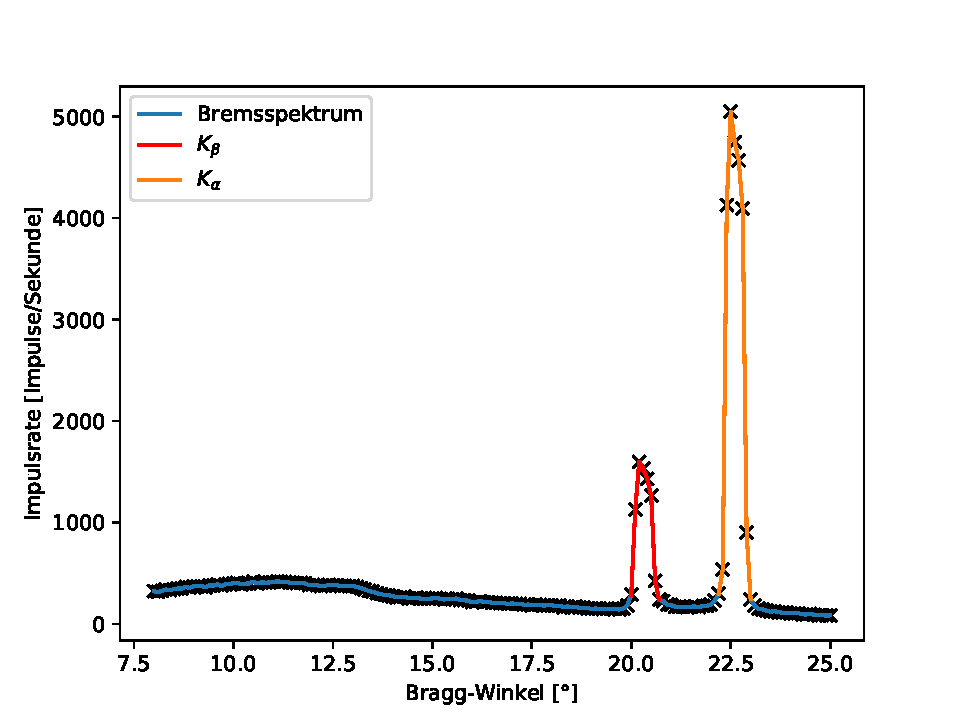
\includegraphics[width = 0.9\linewidth]{Spektrum_Cu.pdf}
            \label{fig:Spektrum}
        \end{figure}
        \FloatBarrier

        Über eine Scipy-Funktion wurden die Maxima der charakteristischen Strahlung wie folgt bestimmt.

        \begin{align}
            &\alpha_{K_{\alpha}} = 22,5°
            &\alpha_{K_{\beta}}  = 20,2°
        \end{align}

        \noindent
        Zum Vergleich mit den Literaturenergien wird diese aus den ermittelten Winkel über die nach E umgestellte Formel \ref{eqn:Bragg} berechnet.

        \begin{align}
            &E = \frac{hc}{2 \cdot d \cdot sin(\alpha)} \qquad \text{mit} \qquad d=201,4\cdot 10^{\left(-12\right)} \, m\\
            &E_{K_{\alpha}} = 8043 \, eV \\
            &E_{K_{\beta}}  = 8914 \, eV
        \end{align}

        \subsection{Wellenlängenabhängigkeit der Transmission}
        \noindent
        Nun wird die Transmission des Aluminiumabsorbers gegen die Wellenlänge aufgetragen. Dazu müssen zum einen die Impulsraten $N_1$ und $N_0$ über die 
        Totzeitkorrektur \ref{eqn:Totzeitkorrektur} in die Intensitäten und der Winkel über die umgestellte Bragg-Bedingung \ref{eqn:Bragglambda} in die 
        Wellenlänge umgerechnet werden. Zuletzt muss die Transmission aus dem Quotienten von  $I_1$ und $I_0$ berechnet werden.

        \begin{equation}
            \lambda = 2dn \cdot sin(\alpha) \qquad \text{mit} \qquad d=201,4\cdot 10^{\left(-12\right)} \, m, \qquad n=1
            \label{eqn:Bragglambda}
        \end{equation}
        \begin{equation}
            T = \frac{I_1}{I_0}
            \label{eqn:Trans}
        \end{equation}
        
        \noindent
        Die gemessenen und korrigierten Werte finden sich ebenfalls im Anhang (ref) und werden nun in einem Diagramm aufgetragen. Zudem wird eine 
        Ausgleichgerade durch die Werte gelegt, die auf folgender Geradengleichung beruht:

        \begin{align}
            T\left(\lambda\right) &= m &\cdot \lambda &+ b\\
            T\left(\lambda\right) &= -15 \cdot 10^{\left(-9\right)} \frac{W}{m³} &\cdot \lambda &+ 1,22 \frac{W}{m²}
            \label{eqn:Regression}
        \end{align}

        \FloatBarrier
        \begin{figure}[h]
            \centering
            \caption{In der Abbildung ist die Wellenlängenabhängigkeit der Transmission des Aluminiumabsorbers zu sehen. Um den linearen Zusammenhang in der Auswertung besser nutzen zu können, wird zudem eine lineare Regression mit angegebenen Parametern \ref{eqn:Regression} über die Messwerte gelegt.}
            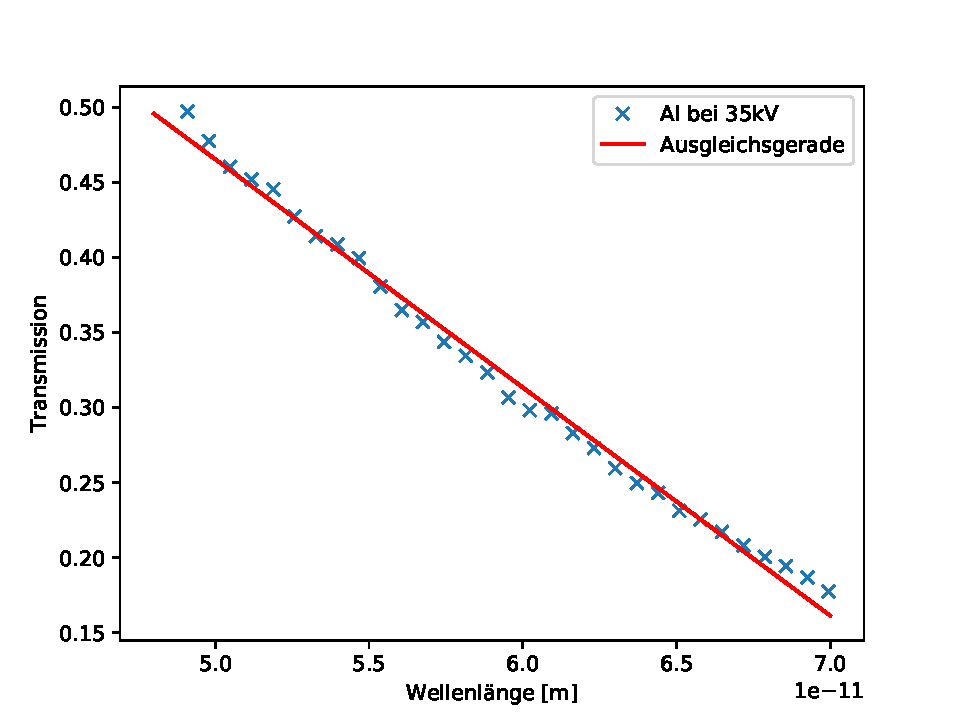
\includegraphics[width = 0.9\linewidth]{Compton_Alu.pdf}
            \label{fig:Transmission}
        \end{figure}
        \FloatBarrier

        \subsection{Bestimmung der Compton-Wellenlänge}
        Mit den nun bereitstehenden Grundlagen wird die Compton-Wellenlänge bestimmt. Indem die Intensitäten von nicht gestreuten $I_{\text{ungestreut}}$ 
        und compton-gestreuten $I_{\text{gestreut}}$ Photonen über Formel \ref{eqn:Trans} in die entsprechende Transmission des Aluminiumabsorbers umgerechnet
        werden. Dabei bezeichnet $I_{\text{norm}}$ die Intensität bei gleichem Streuwinkel ohne Aluminiumabsorber. 
        
        \begin{align}
            T_{\text{ungestreut}} = \frac{I_{\text{ungestreut}}}{I_{\text{norm}}}=0,43\\
            T_{\text{gestreut}} = \frac{I_{\text{gestreut}}}{I_{\text{norm}}}=0,37
            \label{eqn:T1T2}
        \end{align}

        Die den Transmissionen zugehörigen Wellenlängen werden durch Umstellen von \ref{eqn:Regression} nach $\lambda$ und Einsetzen von $T_{\text{ungestreut}}$
        und $T_{\text{gestreut}}$ \ref{eqn:T1T2} ermittelt.

        \begin{align}
            \lambda = \frac{T - 1,22}{-15} \, m \\
            \lambda_{\text{ungestreut}} &= 52,2 \cdot 10^{\left(-12\right)} \, m \\
            \lambda_{\text{gestreut}} &= 56,0 \cdot 10^{\left(-12\right)} \, m
            \label{eqn:y1,y2}
        \end{align}

        Da der Streuwinkkel bei dem Messaufbau 90° beträgt, entspricht die Compton-Wellenlänge $\lambda_{\text{C}}$ der Differenz von $\lambda_{\text{gestreut}}$
        und $\lambda_{\text{ungestreut}}$.
        \begin{align}
            \Delta \lambda &= \lambda_{\text{gestreut}} - \lambda_{\text{ungestreut}} =& \lambda_{\text{c}} \cdot \left(1 -cos (\theta)\right)\\
            \lambda_{\text{c}} &= \lambda_{\text{gestreut}} - \lambda_{\text{ungestreut}} =& 3,8 \cdot 10^{\left(-12\right)} \, m \qquad \text{mit} \qquad \theta=90°
            \label{eqn:ycexp}
        \end{align} 



    \section{Diskussion}


    \newpage
    \section{Literaturverzeichnis}
            [1] \textit{Versuchsanleitung V603 - Compton-Effekt.} TU Dortmund, 2020 \newline
            [2] PHYWE Systeme GmbH \& Co. KG: \textit{Charakteristische Röntgenstrahlungvon Kupfer} 03.Mai.2020
                \url{http://www.phywe-ru.com/index.php/fuseaction/download/lrn_file/versuchsanleitungen/P2540101/d/p2540101d.pdf}

    \newpage
    \section{Anhang}

    \begin{table}[h]
        \centering
        \caption{In der Tabelle sind zum einen die primären Messdaten wie der Bragg-Winkel und die zugehörigen Zählraten mit $N_1$ und ohne Aluminiumabsorber $N_2$. Zusätzlich sind auch die daraus berechneten Größen aufgelistet. Die Wellenlänge wird aus dem Bragg-Winkel berechnet \ref{eqn:Bragglambda}, die Intensitäten $I_0$ und $I_1$ aus den Impulsraten \ref{eqn:Totzeitkorrektur} und die Transmission T wiederum aus eben diesen Intensitäten \ref{eqn:Trans}.}
        \label{tab:Transmission}

        \begin{tabular}{c c c c c c c}
            \toprule
            {Bragg-Winkel [°]}  & {Wellenlänge [pm]} & {$N_0$ [Imp/s]} & {$I_0$ [W/m²]} & {$N_1$ [Imp/s]} & {$I_1$ [W/m²]} & {T} \\ 
            \midrule
            7.0	                &  49,1              &  226.0          &    230,7       &    113,5        &    114,7       &  0,50 \\
            7.1	                &  49,8              &  232.0          &    237,0       &    112,0        &    113,1       &  0,48 \\
            7.2	                &  50,5              &  240.5          &    245,8       &    112,0        &    113,1       &  0,46 \\
            7.3	                &  51,2              &  248.0          &    253,7       &    113,5        &    114,7       &  0,45 \\
            7.4	                &  51,9              &  255.0          &    261,0       &    115,0        &    116,2       &  0,45 \\
            7.5	                &  52,6              &  262.0          &    268,3       &    113,5        &    114,7       &  0,43 \\
            7.6	                &  53,3              &  269.0          &    275,7       &    113,0        &    114,2       &  0,41 \\
            7.7	                &  54,0              &  276.0          &    283,0       &    114,5        &    115,7       &  0,41 \\
            7.8	                &  54,7              &  281.0          &    288,3       &    114,0        &    115,2       &  0,40 \\
            7.9	                &  55,4              &  289.5          &    297,2       &    112,0        &    113,1       &  0,38 \\
            8.0	                &  56,1              &  295.0          &    303,0       &    109,5        &    110,6       &  0,36 \\
            8.1	                &  56,8              &  300.0          &    308,3       &    109,0        &    110,1       &  0,36 \\
            8.2	                &  57,5              &  308.5          &    317,3       &    108,0        &    109,1       &  0,34 \\
            8.3	                &  58,2              &  311.0          &    320,0       &    106,0        &    107,0       &  0,33 \\
            8.4	                &  58,9              &  317.0          &    326,3       &    104,5        &    105,5       &  0,32 \\
            8.5	                &  59,6              &  324.0          &    333,7       &    101,5        &    102,4       &  0,31 \\
            8.6	                &  60,3              &  328.5          &    338,5       &    100,0        &    101,0       &  0,30 \\
            8.7	                &  61,0              &  332.5          &    342,8       &    100,5        &    101,4       &  0,30 \\
            8.8	                &  61,7              &  337.0          &    347,5       &    97,5         &    98,4        &  0,28 \\
            8.9	                &  62,4              &  340.5          &    351,3       &    95,0         &    95,8        &  0,27 \\
            9.0	                &  63,1              &  348.0          &    359,3       &    92,5         &    93,3        &  0,26 \\
            9.1	                &  63,7              &  350.0          &    361,4       &    98,5         &    90,2        &  0,25 \\
            9.2	                &  64,4              &  353.0          &    364,6       &    88,0         &    88,7        &  0,24 \\
            9.3	                &  65,1              &  356.5          &    368,3       &    84,5         &    85,1        &  0,23 \\
            9.4	                &  65,8              &  359.0          &    371,0       &    83,0         &    83,6        &  0,23 \\
            9.5	                &  66,5              &  363.5          &    375,8       &    81,0         &    81,6        &  0,22 \\
            9.6	                &  67,2              &  367.0          &    379,5       &    78,5         &    79,1        &  0,21 \\
            9.7	                &  67,9              &  369.0          &    381,7       &    76,0         &    76,5        &  0,20 \\
            9.8	                &  68,6              &  370.5          &    383,3       &    74,0         &    74,5        &  0,19 \\
            9.9	                &  69,3              &  375.0          &    388,1       &    72,0         &    72,5        &  0,19 \\
            10.0                &  70,0              &  375.5          &    388,6       &    68,5         &    68,9        &  0,18 \\
            \bottomrule
            
        \end{tabular}
        
    \end{table}

\end{document}